\documentclass[border=4pt]{standalone}
\usepackage{fontspec}
\setmainfont{DMSans9pt}[Path=../../fonts/, Extension=.ttf, UprightFont=*-Regular, BoldFont=*-Bold, ItalicFont=*-Italic, BoldItalicFont=*-BoldItalic]
\setsansfont{DMSans9pt}[Path=../../fonts/, Extension=.ttf, UprightFont=*-Regular, BoldFont=*-Bold, ItalicFont=*-Italic, BoldItalicFont=*-BoldItalic]
\usepackage{amsmath,amssymb,xcolor}
\usepackage{tikz}
\usetikzlibrary{arrows.meta,positioning,shapes.geometric,shapes.misc,fit,backgrounds,calc,decorations.pathreplacing,shadows}
\definecolor{cTwo}{HTML}{4C72B0}
\definecolor{cOne}{HTML}{DD8452}
\definecolor{cDetr}{HTML}{55A868}
\definecolor{cOvd}{HTML}{8172B3}
\definecolor{cAgent}{HTML}{C44E52}
\definecolor{cEdge}{HTML}{937860}
\definecolor{cApp}{HTML}{DA8BC3}
\definecolor{cData}{HTML}{4C9BB0}

\makeatletter
\def\refmap#1#2{\expandafter\def\csname rm@#1\endcsname{#2}}
\def\rm@ref#1{\csname rm@#1\endcsname}
\renewcommand{\ref}{\@ifstar\rm@ref\rm@ref}
\renewcommand{\eqref}[1]{(\csname rm@#1\endcsname)}
\makeatother

\refmap{eq:ciou}{10}\refmap{eq:detector}{1}\refmap{eq:dfl}{11}\refmap{eq:giou}{9}\refmap{eq:glip}{17}\refmap{eq:grpo}{20}\refmap{eq:infonce}{15}\refmap{eq:mllm-box}{19}\refmap{eq:ovd}{2}\refmap{eq:reparam}{18}\refmap{eq:roialign}{6}\refmap{eq:rpn}{5}\refmap{eq:siglip}{16}\refmap{eq:tal}{8}\refmap{sec:agentic}{5}\refmap{sec:closed}{3}\refmap{sec:manufacturing}{7.1}\refmap{sec:mllm-direct}{5.1}\refmap{sec:mllm-rl}{5.2}\refmap{sec:mllm-tools}{5.3}\refmap{sec:ovd}{4}\refmap{sec:ovd-distill}{4.2}\refmap{sec:ovd-grounding}{4.3}\refmap{sec:ovd-owl}{4.4}\refmap{sec:ovd-rt}{4.5}\refmap{sec:ovd-unified}{4.6}\refmap{sec:twostage}{3.1}\refmap{sec:vlfound}{4.1}\refmap{sec:yolo}{3.3}\refmap{tab:yolo}{4}
%% ---------- illustrative scene thumbnails (drawn, not photographs); origin = lower-left, size 2.4 x 1.7
\definecolor{pcbG}{HTML}{2E7D4F}\definecolor{pcbD}{HTML}{1F5A39}\definecolor{chipK}{HTML}{2B2B2B}
\definecolor{soil}{HTML}{8B6B4A}\definecolor{soilD}{HTML}{6E5238}\definecolor{crop}{HTML}{6BB04A}\definecolor{weed}{HTML}{3E7C2A}
\definecolor{belt}{HTML}{5A5F66}\definecolor{carton}{HTML}{C9A46A}\definecolor{cartonD}{HTML}{A9844C}\definecolor{pallet}{HTML}{9C7A4F}
\tikzset{bx/.style={draw=#1, line width=0.8pt}, bxl/.style={fill=#1, text=white, font=\fontsize{4.2}{4.2}\selectfont\bfseries, inner sep=0.6pt, anchor=south west}}
% PCB: chips, pads, one solder bridge
\newcommand{\scenePCB}{%
  \fill[pcbG, rounded corners=1pt] (0,0) rectangle (2.4,1.7);
  \foreach \y in {0.25,0.55,0.85,1.15,1.45}{\draw[pcbD, line width=0.35pt] (0.05,\y) -- (2.35,\y);}
  \fill[chipK] (0.25,0.75) rectangle (0.95,1.4);
  \foreach \x in {0.32,0.47,0.62,0.77,0.89}{\fill[gray!60] (\x-0.03,0.66) rectangle (\x+0.03,0.75); \fill[gray!60] (\x-0.03,1.4) rectangle (\x+0.03,1.49);}
  \fill[chipK] (1.35,0.2) rectangle (2.15,0.7);
  \foreach \x in {1.45,1.65,1.85,2.05}{\fill[gray!60] (\x-0.04,0.7) rectangle (\x+0.04,0.8);}
  \fill[gray!70] (1.7,1.05) circle (0.07); \fill[gray!70] (1.95,1.05) circle (0.07); \fill[gray!70] (2.2,1.05) circle (0.07);
  \fill[gray!75] (1.7,1.0) rectangle (1.95,1.1); % bridge between pads
}
% Field: soil rows with crops and weeds
\newcommand{\sceneField}{%
  \fill[soil, rounded corners=1pt] (0,0) rectangle (2.4,1.7);
  \foreach \y in {0.35,0.85,1.35}{\fill[soilD] (0.05,\y-0.06) rectangle (2.35,\y+0.06);}
  \foreach \x/\y in {0.3/0.35,0.8/0.35,1.3/0.35,1.8/0.35,0.3/0.85,0.8/0.85,1.8/0.85,2.2/0.85,0.55/1.35,1.05/1.35,1.55/1.35,2.05/1.35}{%
    \fill[crop] (\x,\y) ellipse (0.11 and 0.07); \fill[crop] (\x,\y+0.05) ellipse (0.05 and 0.1);}
  \foreach \x/\y in {1.3/0.85,0.6/0.6}{\foreach \a in {0,60,...,300}{\fill[weed, rotate around={\a:(\x,\y)}] (\x+0.07,\y) ellipse (0.07 and 0.025);}}
}
% Warehouse: belt with cartons and a pallet stack
\newcommand{\sceneWarehouse}{%
  \fill[gray!15, rounded corners=1pt] (0,0) rectangle (2.4,1.7);
  \fill[belt] (0,0.15) rectangle (2.4,0.45);
  \foreach \x in {0.1,0.5,...,2.3}{\draw[gray!50, line width=0.3pt] (\x,0.15) -- (\x,0.45);}
  \fill[carton] (0.2,0.45) rectangle (0.75,0.85); \draw[cartonD] (0.475,0.45) -- (0.475,0.85);
  \fill[carton] (1.0,0.45) rectangle (1.4,0.75); \draw[cartonD] (1.2,0.45) -- (1.2,0.75);
  \fill[pallet] (1.6,0.55) rectangle (2.3,0.65);
  \fill[carton] (1.62,0.65) rectangle (1.95,0.95); \fill[carton] (1.97,0.65) rectangle (2.28,0.95); \fill[carton] (1.75,0.95) rectangle (2.15,1.25);
  \draw[cartonD] (1.62,0.65) rectangle (1.95,0.95); \draw[cartonD] (1.97,0.65) rectangle (2.28,0.95); \draw[cartonD] (1.75,0.95) rectangle (2.15,1.25);
}
% Metal surface with scratch and dent
\newcommand{\sceneSurface}{%
  \shade[left color=gray!35, right color=gray!15, rounded corners=1pt] (0,0) rectangle (2.4,1.7);
  \foreach \i in {1,...,14}{\draw[gray!45, line width=0.2pt] (0.05,0.1*\i) -- (2.35,0.1*\i+0.03);}
  \draw[gray!80!black, line width=0.6pt] (0.4,1.25) .. controls (0.8,1.15) and (1.0,1.05) .. (1.35,0.95);
  \fill[gray!65] (1.8,0.45) ellipse (0.16 and 0.1);
}

\begin{document}
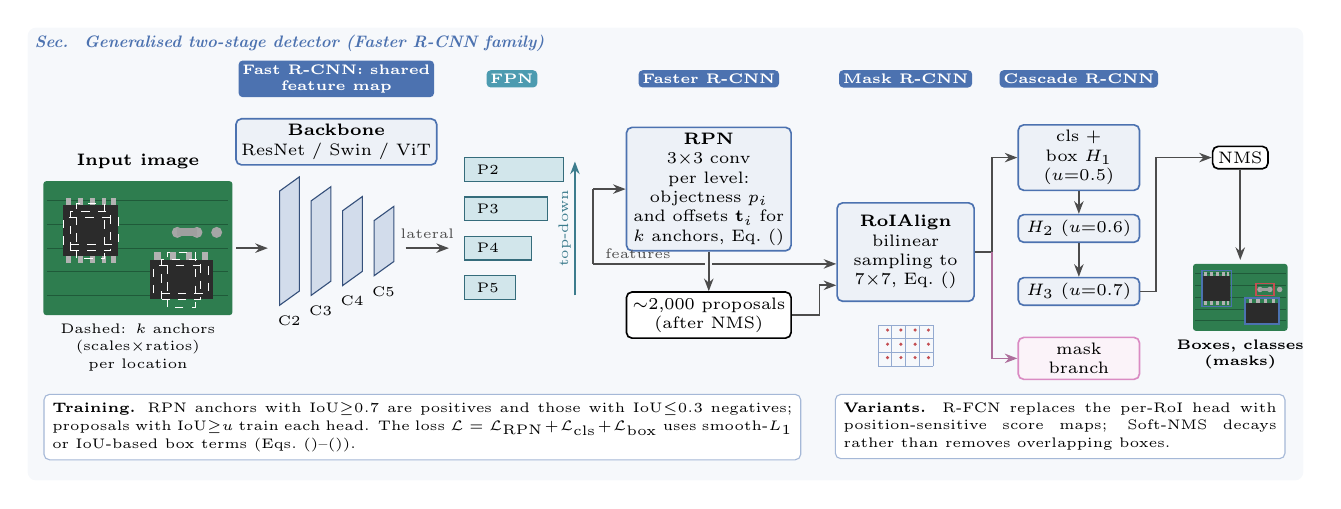
\begin{tikzpicture}[
  font=\fontsize{6}{7}\selectfont,
  mod/.style={draw=#1, fill=#1!10, rounded corners=2pt, line width=0.6pt, align=center, inner sep=2pt},
  tag/.style={fill=#1, text=white, rounded corners=1.5pt, font=\fontsize{5.2}{6}\selectfont\bfseries, inner sep=1.4pt, align=center},
  sec/.style={font=\fontsize{6.2}{7}\selectfont\bfseries\itshape, text=#1, anchor=north west, inner sep=1pt},
  fm/.style={draw=#1!70!black, fill=#1!25, line width=0.4pt},
  arr/.style={-{Stealth[length=1.6mm]}, line width=0.6pt, black!70},
  note/.style={font=\fontsize{5.4}{6.4}\selectfont, align=justify, text width=#1, inner sep=0pt},
]
\fill[cTwo!5, rounded corners=3pt] (-0.2,-0.75) rectangle (16.0,5.0);
\node[sec=cTwo] at (-0.15,4.95) {Sec.~\ref*{sec:twostage} Generalised two-stage detector (Faster R-CNN family)};
% ---------- input
\begin{scope}[shift={(0,1.35)}]
  \scenePCB
  \foreach \x/\y in {0.6/1.07,1.75/0.45}{\foreach \w/\h in {0.5/0.5,0.7/0.35,0.35/0.7}{\draw[white, dashed, line width=0.35pt] (\x-\w/2,\y-\h/2) rectangle (\x+\w/2,\y+\h/2);}}
\end{scope}
\node[font=\fontsize{6}{7}\selectfont\bfseries] at (1.2,3.3) {Input image};
\node[note=2.4cm, align=center, anchor=north] at (1.2,1.25) {Dashed: $k$ anchors (scales${\times}$ratios) per location};
\draw[arr] (2.45,2.2) -- (2.85,2.2);
% ---------- backbone C2-C5
\foreach \i/\h in {0/1.45,1/1.2,2/0.95,3/0.7}{
  \fill[fm=cTwo] (3.0+\i*0.4,2.2-\h/2) -- ++(0.25,0.18) -- ++(0,\h) -- ++(-0.25,-0.18) -- cycle;
  \node[font=\fontsize{4.8}{5}\selectfont] at (3.12+\i*0.4,2.2-\h/2-0.2) {C\the\numexpr\i+2\relax};}
\node[mod=cTwo, minimum width=1.9cm] at (3.72,3.55) {\textbf{Backbone}\\ResNet / Swin / ViT};
\node[tag=cTwo] at (3.72,4.35) {Fast R-CNN: shared\\feature map};
% ---------- FPN
\draw[arr] (4.6,2.2) -- node[above, font=\fontsize{4.6}{5}\selectfont]{lateral} (5.15,2.2);
\foreach \i/\w in {0/1.25,1/1.05,2/0.85,3/0.65}{
  \fill[fm=cData] (5.35,3.05-\i*0.5) rectangle ++(\w,0.3);
  \node[font=\fontsize{4.8}{5}\selectfont, anchor=west] at (5.38,3.2-\i*0.5) {P\the\numexpr\i+2\relax};}
\draw[arr, cData!80!black] (6.75,1.6) -- (6.75,3.3) node[midway, sloped, above, font=\fontsize{4.6}{5}\selectfont, inner sep=1.2pt] {top-down};
\node[tag=cData] at (5.95,4.35) {FPN};
% ---------- RPN
\node[mod=cTwo, minimum height=1.25cm, text width=1.95cm] (rpn) at (8.45,2.95) {\textbf{RPN}\\$3{\times}3$ conv per level:\\objectness $p_i$ and offsets $\mathbf{t}_i$ for $k$ anchors, Eq.~(\ref*{eq:rpn})};
\node[tag=cTwo] at (8.45,4.35) {Faster R-CNN};
\node[mod=black, fill=white, text width=1.95cm] (prop) at (8.45,1.35) {${\sim}$2{,}000 proposals (after NMS)};
\draw[line width=0.6pt, black!70] (6.98,2.0) -- (6.98,2.95);
\draw[arr] (6.98,2.95) -- (rpn.west);

% ---------- RoIAlign
\node[mod=cTwo, minimum height=1.25cm, text width=1.6cm] (roi) at (10.95,2.15) {\textbf{RoIAlign}\\bilinear sampling to $7{\times}7$, Eq.~(\ref*{eq:roialign})};
\begin{scope}[shift={(10.6,0.7)}]
  \draw[cTwo!60, line width=0.3pt] (0,0) grid[step=0.175] (0.7,0.525);
  \foreach \x/\y in {0.09/0.09,0.26/0.09,0.44/0.09,0.61/0.09,0.09/0.26,0.26/0.26,0.44/0.26,0.61/0.26,0.09/0.44,0.26/0.44,0.44/0.44,0.61/0.44}{\fill[cAgent] (\x+0.03,\y+0.02) circle (0.022);}
\end{scope}
\node[tag=cTwo] at (10.95,4.35) {Mask R-CNN};
\draw[arr] (prop.east) -- ++(0.35,0) |- ([yshift=-12pt]roi.west);
\draw[arr] (6.98,2.0) -- (roi.west |- 0,2.0) node[pos=0.03, above right, font=\fontsize{4.6}{5}\selectfont, inner sep=1.5pt]{features};
\draw[arr, preaction={draw=cTwo!5, line width=2.6pt, -}] (rpn.south) -- (prop.north);
% ---------- heads
\node[mod=cTwo, text width=1.4cm] (h1) at (13.15,3.35) {cls + box $H_1$\\($u{=}0.5$)};
\node[mod=cTwo, text width=1.4cm] (h2) at (13.15,2.45) {$H_2$ ($u{=}0.6$)};
\node[mod=cTwo, text width=1.4cm] (h3) at (13.15,1.65) {$H_3$ ($u{=}0.7$)};
\node[mod=cApp, text width=1.4cm] (mk) at (13.15,0.8) {mask branch};
\coordinate (sp) at (12.05,2.15);
\draw[line width=0.6pt, black!70] (roi.east) -- (sp);
\draw[arr] (sp) |- (h1.west);
\draw[arr] (h1.south) -- (h2.north); \draw[arr] (h2.south) -- (h3.north);
\draw[arr, cApp!80!black] (sp) |- (mk.west);
\node[tag=cTwo] at (13.15,4.35) {Cascade R-CNN};
% ---------- output
\node[mod=black, fill=white] (nms) at (15.2,3.35) {NMS};
\draw[arr] (h3.east) -- ++(0.2,0) |- (nms.west);
\begin{scope}[shift={(14.6,1.15)}, scale=0.5]
  \scenePCB
  \draw[bx=cTwo, line width=0.6pt] (0.22,0.62) rectangle (0.98,1.53);
  \draw[bx=cTwo, line width=0.6pt] (1.32,0.17) rectangle (2.18,0.83);
  \draw[bx=cAgent, line width=0.6pt] (1.6,0.9) rectangle (2.05,1.2);
\end{scope}
\draw[arr] (nms.south) -- (15.2,2.05);
\node[font=\fontsize{5.4}{6}\selectfont\bfseries, align=center] at (15.2,0.85) {Boxes, classes\\(masks)};
% ---------- bottom notes
\node[draw=cTwo!50, fill=white, rounded corners=2pt, note=9.4cm, inner sep=3pt, anchor=north west] at (0,0.35) {\textbf{Training.} RPN anchors with IoU${\ge}0.7$ are positives and those with IoU${\le}0.3$ negatives; proposals with IoU${\ge}u$ train each head. The loss $\mathcal{L}=\mathcal{L}_{\text{RPN}}+\mathcal{L}_{\text{cls}}+\mathcal{L}_{\text{box}}$ uses smooth-$L_1$ or IoU-based box terms \mbox{(Eqs.~(\ref*{eq:giou})--(\ref*{eq:ciou}))}.};
\node[draw=cTwo!50, fill=white, rounded corners=2pt, note=5.5cm, inner sep=3pt, anchor=north west] at (10.05,0.35) {\textbf{Variants.} R-FCN replaces the per-RoI head with position-sensitive score maps; Soft-NMS decays rather than removes overlapping boxes.};
\end{tikzpicture}

\end{document}
